\chapter{Evaluation}

This chapter details the tests performed on the Visibility field computation code. The first test shows the difference in computation time between volumes of differing dimensions. The second test compared the computation times for the same volume but with the alpha values within the transfer function changed. The final test altered the size of the local work group within the compute shader to determine the impact on performance.

For each of these tests, the speed was computed as an average over 360 frames, where the volume was rotated 1 degree each time. The measurement was taken using the system clock, and measured only the time it took to setup, call the Compute Shader and then wait for it to return.

The measurements were taken on a GTX 720 on a desktop running an average 

\section{Data Used}

The tests detailed below use five different data volumes. These are listed below.

\begin{table}

\begin{center}
\begin{tabular}{l|c}
Data Set & Dimensions (x * y * z) \\
\hline
\hline
Knee & 379 * 229 * 305 \\
Bonsai & 256 * 256 * 256 \\
Engine & 256 * 256 * 110 \\
Tooth & 140 * 120 * 161 \\
Nucleon & 41 * 41 * 41 
\end{tabular}
\end{center}
\caption{\textit{List of data sets used and their size}}
\end{table}

The same transfer function was used for each test, with the exception of  the second test. In this case, new transfer functions were created by reducing the opacities for the original transfer function by a fraction. The transfer function with the lowest opacity values had been assigned values $\frac{1}{4}$ of those from the original, the next with $\frac{1}{2}$, and the final with $\frac{3}{4}$. 

\section{Change in Computation Time against Volume Size}

The aim of this test was to determine whether the computation time of the visibility field changed with a change in the size of the data set, and if so by how much. As shown in the table above, there was a good variety of sizes to test with, and the test resulted in the graph below. As would be expected, the graph suggests a linear relationship between average computation time and the size of the data set. The y-intercept is approximately 15ms, the time it took for the compute shaders to be set up and return the final values.

\begin{figure}[H]
\centering
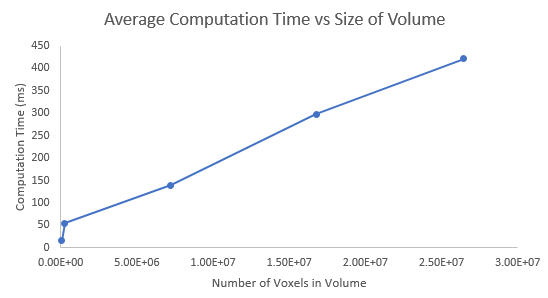
\includegraphics[scale=1.0]{sizes.PNG} 
\caption{\textit{A graph of the average computation times against the size of the data set being worked with}}
\end{figure}

\section{Change in Computation Time against Opacity}

Within the shader code, there is an early exit in the case where the code determines that the voxel is no longer visible behind all the other voxels in front of it. The aim of this test was to determine whether the computation time of the visibility field would change if the opacities of the voxels was changed, and perhaps cause the early exit to be used less often. This was achieved by measuring the speed of the computation against the same transfer function, but each copy of the transfer function having a successively lower opacity value for the most common intensity value over all the data sets. The results are shown below. The data suggests that there could be a small increase with lower opacities for certain intensity values, but the results are inconclusive, given how small the change is.

\begin{figure}[H]
\centering
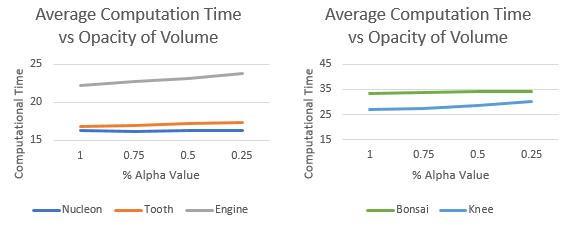
\includegraphics[scale=1.0]{alphaValues} 
\caption{\textit{A graph of the average computation times for each version of the transfer function over a total of 360 frames.}}
\end{figure}

\section{Change in Computation Time against Local Work Group Size}

The impact of the Local Work Group size on the Computation time was an unknown factor within this project. This test was designed to determine whether varying this size had any effect. It was evaluated by measuring the speed of the computation of the visibility field for different sizes of local group. The results are shown in figure 5.1 below. The data points to an exponential decrease in the computation time with an increase in workgroup size in powers of 2.

\begin{figure}[H]
\centering
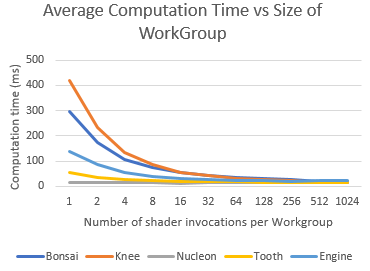
\includegraphics[scale=1.0]{workgroupSize} 
\caption{\textit{A graph of the average computation times for each work group size over a total of 360 frames.}}
\end{figure}

One interesting observation that was made was on the errors that cropped up within the volume during evaluation during this test. While varying the size of each dimension disproportionally had no visible difference from varying each dimension equally, it was noticed that sometimes if a single dimension was large enough, errors would occur in the creation of the visibility field. In the case of the Engine data set, the volume would no longer output a visibility field if the value for the X dimension for the work group exceeded 256, while it would only output a partial visibility field for certain values of Z. This effect was also observed on the results from the saliency field compute shader.

The causes of thes errors was discovered when the sizes of each volume were determined. The tests were performed with volumes where each dimension was a power of 2. However, in table 5.1, very few of the volumes have power of 2 dimensions. In the case of the Engine, its length is 255 voxels, meaning that when it was no longer fully rendering, it meant that the compute shader had gotten too large. 

The partial rendering error can also be explained with the size of the volumes. Since the Z dimension is the smallest, and the volume is aligned on that axis, the error was most noticeable there, but still present on the other axes. When assigning data points to a compute shader, the program divide the volume's dimensions by the size of the work group to get the number of data points per work group. However, since it rounds down, if there is any remainder from the division, those points will not be assigned to a workgroup. With a small workgroup or a large remainder, this effect is more noticeable, but will be present in any data sets whose dimensions won't have many numbers that divide into them evenly. Figure 5.3 was created using work group sizes that minimised this error as much as possible, but it will still be present in any volumes whose dimensions are not a power of 2.

\begin{figure}[H]
\centering
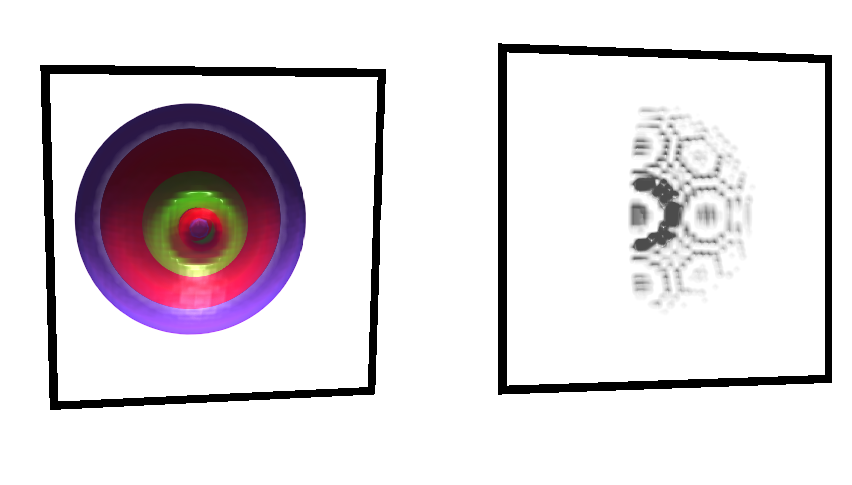
\includegraphics[scale=0.6]{nucleon_error} 
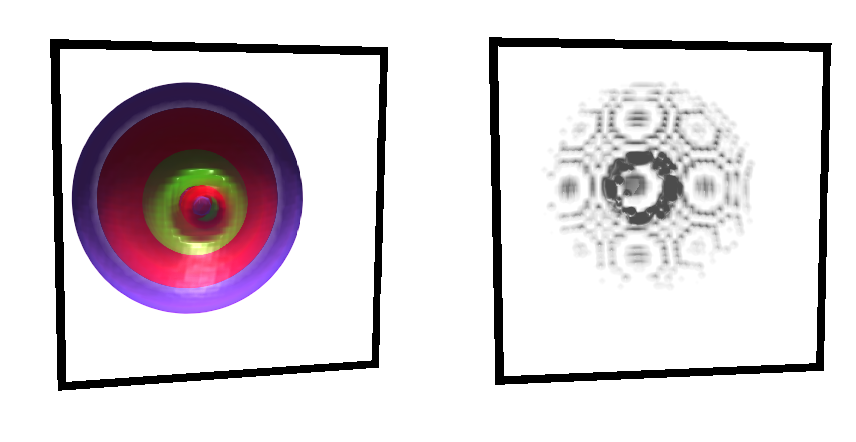
\includegraphics[scale=0.6]{nucleon_fine} 
\caption{\textit{Images showing the result of making the workgroup's x dimension equal to 20, thus cutting off most of the data, compared to making it equal to 41, which is the same as the volume's own dimension}}
\end{figure}
